\chapter{Theory and Fundamentals of MIMO and MCM}
This chapter focuses on the fundamental principles of \acrshort{mimo} and \acrshort{mcm}. We firmly establish some of the prerequisite learning required before we can discuss the actual design of our system in the next chapter. We begin by looking at the shortcomings of single channel systems and how they can be overcome with the help of \acrshort{mcm}. We also highlight how some of the shortcomings of single channel systems can be used to our advantage in \acrshort{mcm}-\acrshort{mimo} systems. We also spend some time looking into concepts such as \gls{rayleigh fading} and Alamouti coding scheme to gain a thorough understanding on mobile communication systems.

\section{The Need of MCM and MIMO}
\subsection{Fading and Diversity}
\subsubsection{Fading and Path Loss}
In a typical mobile communication system, the \acrlong{ue} abbreviated as \acrshort{ue} and \acrlong{bs} abbreviated as \acrshort{bs} are quite far apart. Typical distances are in the kilometer range. As a result, the signal undergoes attenuation as it travels and signal quality degrades to levels that make retrieval of information impossible. A typical example of the variation of received power with distance is given in the figure \ref{fig:path loss}.\\
Various statistical models have been developed to model path loss and fading. In our report, we use a simple \acrlong{los} path loss function abbreviated as \acrshort{los}. This coupled with \gls{rayleigh fading} and \acrshort{awgn} noise forms the channel component of our report. The exact implementation details of each of these terms is discussed in Chapter 3.  
\begin{figure}[!htbp]
\centering
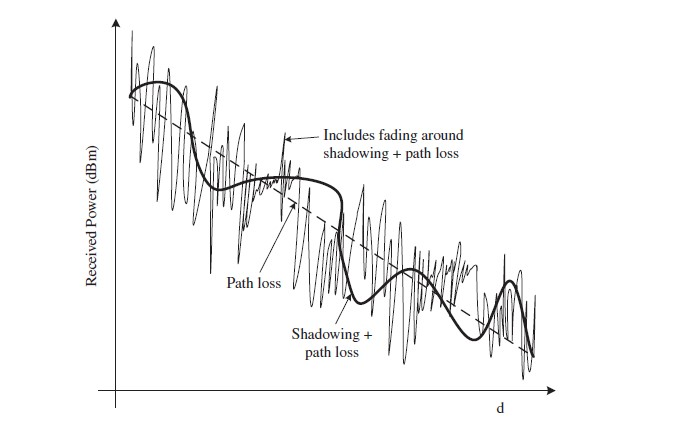
\includegraphics[scale=1]{Chapter 2/Figures/Path Loss}
\caption[Signal Degradation due to Path Loss and Fading]{Variation of Received Signal Power with Distance of separation (d) between transmitter and receiver}
\label{fig:path loss}
\end{figure}
\subsubsection{Diversity}
Mitigation of fading requires techniques such as diversity, wherein copies of the same data are sent from the transmitter to the receiver so that reliability of atleast one copy reaching the receiver in an error free manner is increased.\\
Diversity can be achieved primarily in three ways, they are
\begin{enumerate}
\item \textbf{Frequency Diversity}: Where multiple copies of the same data are sent on different frequency channels
\item \textbf{Time Diversity}: Where multiple copies of the same data are sent at different instances of time
\item \textbf{Spatial Diversity}: Where multiple copies of the same data are sent along different antenna paths.
\end{enumerate}
Among the three possible methods, \gls{spatial diversity} is attractive to us because, the multiple reflections that a signal undergoes in a typical urban setup already provides us with the required diversity without the loss of bandwidth efficiency. Hence, when we refer to diversity, unless otherwise mentioned, it is assumed to refer to \gls{spatial diversity}. A simplified illustration of multipath propagation in urban setting is shown in the figure \ref{fig:multipath propagation}\\
\begin{figure}[!htbp]
\centering
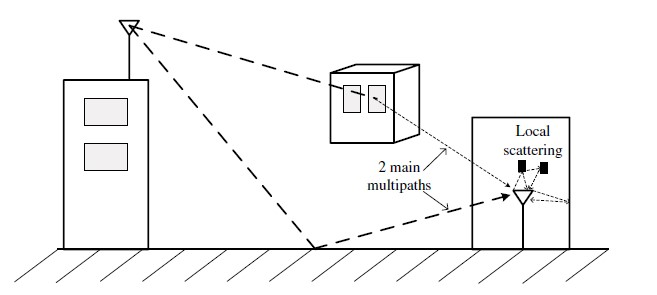
\includegraphics[scale=1]{Chapter 2/Figures/Multipath Propagation}
\caption{Multipath Propagation in a typical urban setting}
\label{fig:multipath propagation}
\end{figure}
However, in a single channel system, the multiple copies arriving at different time instances leads to interference of the signal. This interference may be constructive or destructive in nature as shown in the figure \ref{fig:constructive and destructive interference}. This can lead to difficulties in decoding as it would mean the requirement of expensive equalizers or reduction in the symbol rate. Neither option is feasible for us, and hence, it becomes apparent to us how having multiple transmit and receive antennas can easily overcome this issue. With the help of multiple antennas, the same situation which was causing \acrlong{isi} abbreviated as \acrshort{isi} becomes a boon to us by allowing multiple antenna paths between the transmitter and receiver allowing for easy implementation of \gls{spatial diversity}. This situation is shown in the figure \ref{fig:spatial diversity}\\
As an added benefit, supposing the channel conditions are suitable and the \acrshort{snr} is sufficiently high, instead of sending multiple copies of the same data, we can send different data blocks on different antenna paths increasing the overall data rate per user and the user capacity of the system. This concept is known as \gls{spatial multiplexing} demonstrated in the figure \ref{fig:spatial multiplexing}.
\begin{figure}[!htbp]
\centering
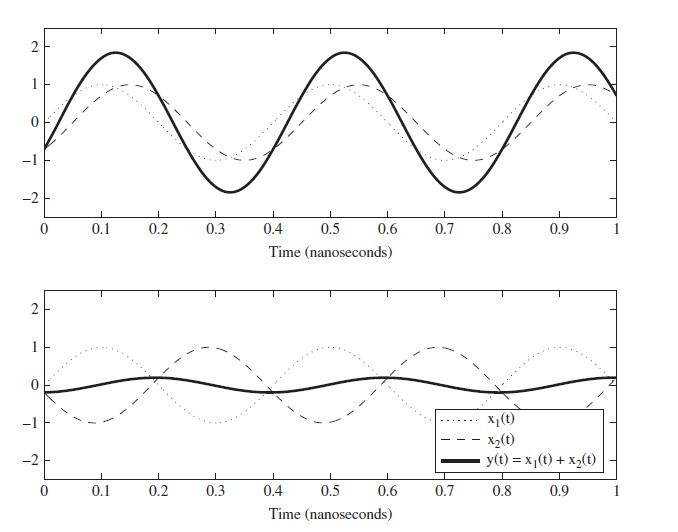
\includegraphics[scale=1]{Chapter 2/Figures/Interference}
\caption[Constructive and Destructive Interference of Signals]{Constructive and Destructive Interference leading to large variation in received signal power.}
\label{fig:constructive and destructive interference}
\end{figure}

\begin{figure}[!htbp]
\centering
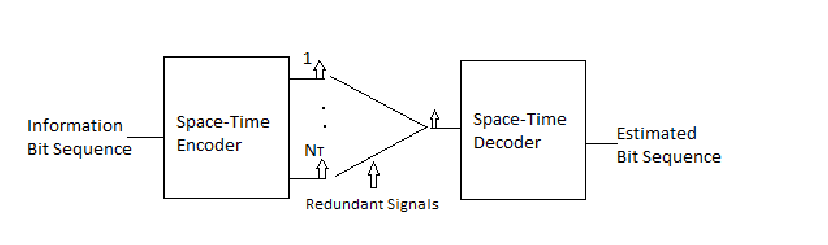
\includegraphics[scale=0.6]{Chapter 2/Figures/Spatial Diversity}
\caption{Spatial Diversity}
\label{fig:spatial diversity}
\end{figure}
\begin{figure}[!htbp]
\centering
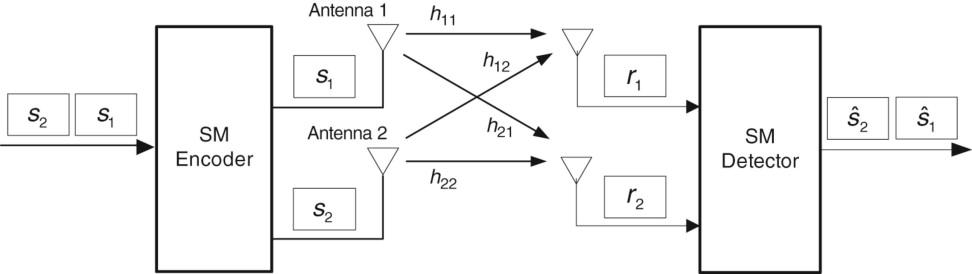
\includegraphics[scale=0.7]{Chapter 2/Figures/Spatial Multiplexing}
\caption{Spatial Multiplexing}
\label{fig:spatial multiplexing}
\end{figure}
\section{Intersymbol Interference, Frequency Selective Fading and the need for MCM}
In the previous section we showed how \acrshort{isi} and fading proved as sufficient motivation to move in the direction of multiple antenna system. However, the issue of \acrshort{isi} cannot be tackled alone by \acrshort{mimo}. Added to the menace of \acrshort{isi} the channel can also degrade the message in a frequency selective manner leading to added difficulties in information recovery at the receiver as shown in the figure \ref{fig:frequency selective fading}. Frequency selective fading occurs because the channel conditions are in constant flux and the message time period is not the same as the time period for which the channel conditions are relatively constant\\
An effective way to combat frequency selective fading is to breakup the entire bandwidth into smaller subchannels where the bandwidth of each subchannel is smaller than \acrshort{bc} the \acrlong{bc}, thus ensuring that the message time period is smaller than \acrshort{td} the \acrlong{td}. This approach to communication is called as Multi Carrier Modulation technique. The implementation of \acrshort{mcm} is simple is we realize that we realize that we can split the given bandwidth into subchannels by simply introducing an \acrshort{ifft} block at the transmitter and to achieve the opposite effect introduce an \acrshort{fft} block at the receiver. With the help of this, we are able to significantly reduce the problems of frequency selective fading and \acrshort{isi}. The basic structure of a \acrshort{mcm} transmitter and receiver is given in the figures \ref{fig:mcm transmitter} and \ref{fig:mcm receiver}.

\begin{figure}[!htbp]
\centering
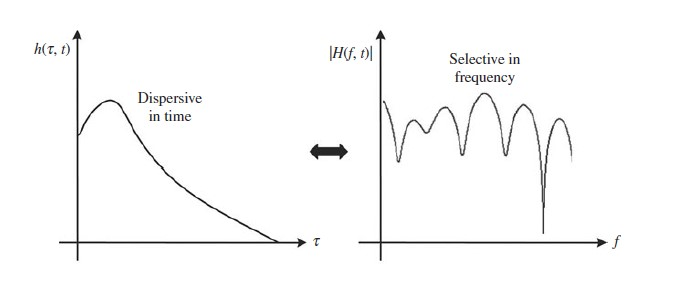
\includegraphics[scale=1]{Chapter 2/Figures/Frequency Selective Fading}
\caption[Frequency Selective Fading]{Frequency Selective Fading which occurs because the message is longer than the delay spread of the channel.}
\label{fig:frequency selective fading}
\end{figure}

\begin{figure}[!htbp]
\centering
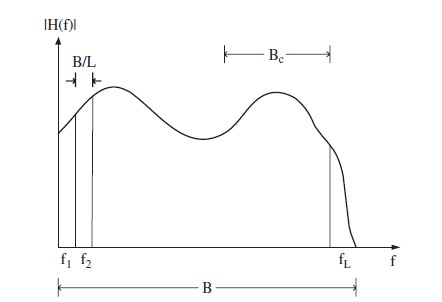
\includegraphics[scale=1]{Chapter 2/Figures/Flat Fading Subchannel}
\caption[Flat Fading Subchannel]{By breaking the large bandwidth into smaller subchannels, we can achieve an almost flat fading subchannel which is desirable.}
\label{fig:flat fading subchannel}
\end{figure}

\begin{figure}[!htbp]
\centering
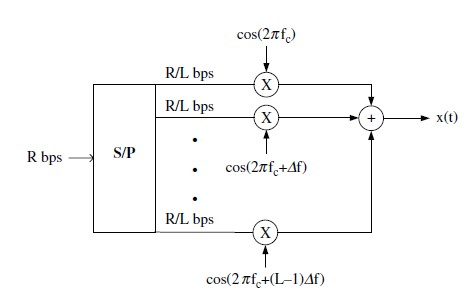
\includegraphics[scale=1]{Chapter 2/Figures/MCM Transmitter}
\caption[MCM Transmitter]{An MCM transmitter with an IFFT block to split the given bandwidth into smaller $L$ subchannels.}
\label{fig:mcm transmitter}
\end{figure}

\begin{figure}[!htbp]
\centering
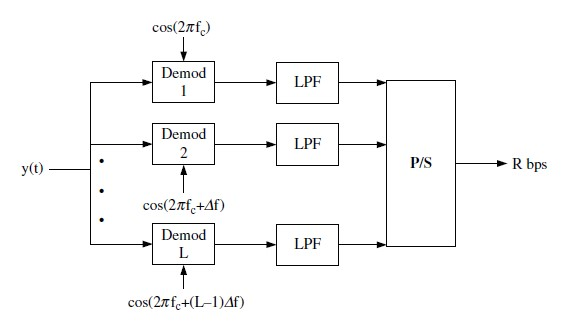
\includegraphics[scale=1]{Chapter 2/Figures/MCM Receiver}
\caption[MCM Receiver]{An MCM transmitter with an FFT block to reverse the effects of IFFT block at the transmitter.}
\label{fig:mcm receiver}
\end{figure}




\section{Shortcomings of MCM and the need for OFDM}
Having shown the implementation of a simple \acrshort{mcm} system, we address some of the shortcomings of this. Primarily,
\begin{itemize}
\item It is impossible to realistically have sharply defined bandwidths, as there exists no way to define a pulse which is strictly rectangular in the frequency domain.
\item Expensive low pass filters will be necessary to maintain orthogonality of the subchannels.
\item Importantly, multiple \acrshort{rf} units are required at both ends for the system to work. This setup, as a result becomes unfeasible and thus, in the next section we look into the \acrshort{ofdm} scheme as an alternative to simple \acrshort{mcm}.
\end{itemize}

\section{OFDM}
\subsection{Concept of OFDM}
\acrlong{ofdm} is a multiplexing scheme where different data symbols are modulated to different frequencies. These frequencies are chosen such that they are all orthogonal. Hence a given instance, only one wave is at it's peak while the rest are at zero allowing us to read the data bits without any \acrlong{isi}. This situation is shown in the figure \ref{fig:ofdm orthogonal waves}.\\

Therefore, we club the different data bits into one block called an \acrshort{ofdm} symbol. To avoid \acrshort{isi} between the \acrshort{ofdm} symbols themselves, there is a small time delay introduced between the \acrshort{ofdm} symbols called as \acrlong{tg} which is abbreviated to \acrshort{tg}. It is important that this delay, is atleast as large as the \acrlong{td}.\\
We know that the wireless channel behaves as a \acrlong{lti} system and hence, the channel coefficient and data bits are linearly convolved together whenever a message is passed through it. However, we know that, circular convolution in the time domain yields simple multiplication in the frequency domain. This multiplication is desirable as it leads to simplified computation at the transmitter and receiver. A simple way to covert this linear convolution to circular convolution is to add redundant bits known as \gls{cyclic prefix}. This cyclic prefix is just copying the last $L$ bits of the \acrshort{ofdm} symbol and adding it to the beginning of the symbol. These $L$ bits are transmitted during the time \acrshort{tg} and hence will be lost due to interference between the \acrshort{ofdm} symbols.\\

\begin{figure}[!htbp]
\centering
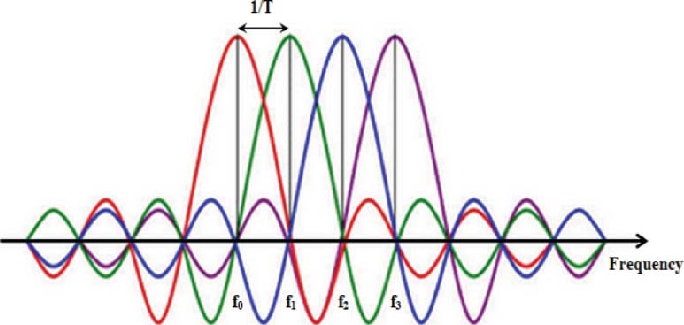
\includegraphics[scale=1]{Chapter 2/Figures/OFDM Orthogonality}
\caption[Orthogonality in OFDM]{An OFDM symbol where different coloured waves correspond to different bits. Notice how when one wave peaks, all the other waves are at their null points.}
\label{fig:ofdm orthogonal waves}
\end{figure}

\begin{figure}[!htbp]
\centering
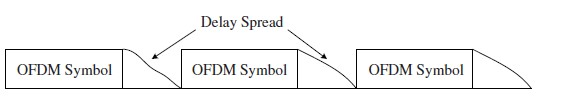
\includegraphics[scale=1]{Chapter 2/Figures/OFDM Symbol Timing}
\caption[Guard Time between OFDM symbols]{A delay of \acrshort{tg} is introduced between the symbols to avoid interference between the \acrshort{ofdm} symbols. Notice that this does not do anything to combat \acrshort{isi} within the \acrshort{ofdm} symbol itself.}
\label{fig:ofdm symbol timing}
\end{figure}

\begin{figure}[!htbp]
\centering
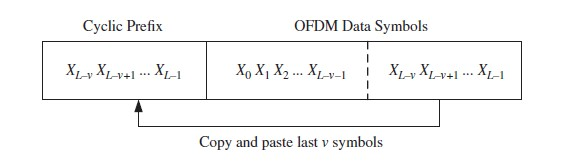
\includegraphics[scale=1]{Chapter 2/Figures/Cyclic Prefix}
\caption[Cyclic Prefix]{The cyclic prefix in an \acrshort{ofdm} symbol.}
\label{fig:ofdm cyclic prefix}
\end{figure}



\subsection{Advantages of OFDM}
Some of the advantages of \acrshort{ofdm} compared to traditional \acrshort{fdm} are as follows.
\begin{itemize}
\item There is no need for any guard bands between carriers leading to higher spectral efficiency.
\item Higher data rates can be achieved as symbol rate need not be lowered for the sake of \acrshort{isi}.
\item System is more robust to multipath effects.
\end{itemize}

\subsection{Disadvantages of OFDM}
\acrshort{ofdm} also comes with a few disadvantages chief among them is the issue of high \acrshort{papr}. Discussing the ways to mitigate this issue is outside the scope of this report and the reader is encouraged to refer to literature such as \parencite{Ghosh2010} to gain a better understanding.

\section{OFDM Transceiver System}
After having seen the motivation for the development of \acrshort{mcm}, \acrshort{mimo} and \acrshort{ofdm} schemes and also having seen a basic \acrshort{mcm} transceiver system, we will combine all the concepts to create an \acrshort{ofdm} transceiver which is capable of sending and receiving data bits packaged in \acrshort{ofdm} symbols.\\
In figure \ref{fig:ofdm transmitter} we see how normal \acrshort{qam} modulated symbols are passed through an \acrshort{ifft} block to assign them to different frequency subchannels. Additional cyclic prefix is added before converting the parallel streams to a serial stream and transmitting it.\\
The \acrshort{ofdm} receiver in figure \ref{fig:ofdm receiver} on the other hand does the exact opposite process, where the received symbols are demodulated according to their respective frequencies and passed through an \acrshort{fft} block to undo the \acrshort{ifft} process. Then, it the demodulated symbols are passed through a \acrlong{mli} detector to get back the information bits.\\

\begin{figure}[!htbp]
\centering
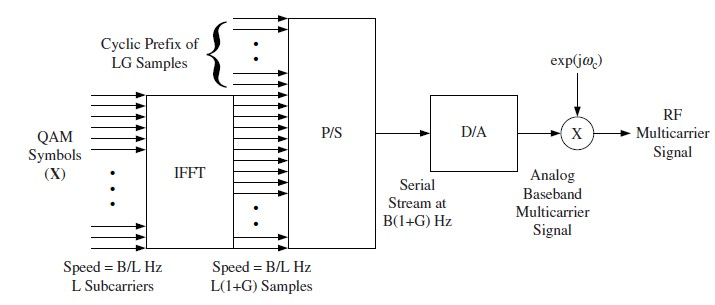
\includegraphics[scale=1]{Chapter 2/Figures/OFDM Transmitter}
\caption{\acrshort{ofdm} Transmitter}
\label{fig:ofdm transmitter}
\end{figure}

\begin{figure}[!htbp]
\centering
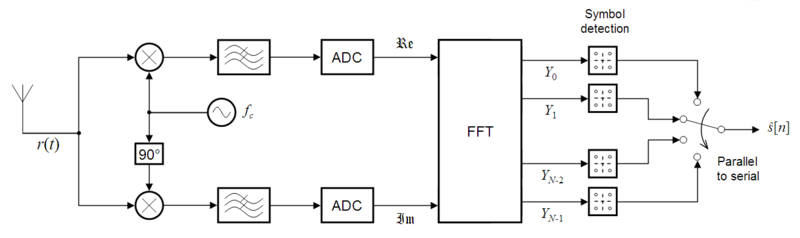
\includegraphics[scale=0.6]{Chapter 2/Figures/OFDM Receiver}
\caption{\acrshort{ofdm} Receiver}
\label{fig:ofdm receiver}
\end{figure}


\section{Alamouti Coding Scheme}
Alamouti coding scheme is a simple coding scheme designed for the purpose of achieving \gls{spatial diversity} in \acrshort{miso} systems. The advantage of this coding scheme is that the transmitter need not know the channel information before sending the data. We describe the coding scheme in this section.\\
Consider two transmitting antennas $T_1$ and $T_2$ and one receiving antenna $R$.\\
Let $h_1$ be the channel coefficient of the first antenna path and $h_2$ be the channel coefficient of the second antenna path.\\
Let $x_1$ and $x_2$ be transmitted by antennas $T_1$ and $T_2$ respectively at a given time instance, and ${-x_2}^*$, ${-x_1}^*$ be the data transmitted in the next time instance by the antennas respectivey.\\
We know that the wireless channel behaves as an \acrshort{lti} system which performs convolution of the data bits and the channel coefficient. Also, let $w_1$ and $w_2$ be the noise vectors added at the two time instances respectively.\\
This situation can be represented mathematically as follows.
\begin{align*}
y_1 &= 
\begin{bmatrix}
h_1&h_2
\end{bmatrix}
\times
\begin{bmatrix}
x_1\\
x_2
\end{bmatrix}
+ w_1\\
y_2 &=
\begin{bmatrix}
h_1&h_2
\end{bmatrix}
\times
\begin{bmatrix}
{-x_2}^*\\
x_1^*
\end{bmatrix}
+w_2
\end{align*}
This can be further simplified as,\\
\begin{align*}
y &= \begin{bmatrix}
y_1\\
y_2^*
\end{bmatrix}
= c_1x_1 + c_2x_2 + w
\end{align*}
Where,
\begin{align*}
c_1&=\begin{bmatrix}
h_1\\
h_2^*
\end{bmatrix}\\
c_2&=\begin{bmatrix}
h_2\\
-h_1^*
\end{bmatrix}
\end{align*}
Here $c_1$ and $c_2$ can be shown as orthogonal in nature and so, this coding scheme is also known as \acrlong{ostbc} scheme.\\
At the receiver, once we have matrix $y$, $x_1$ and $x_2$ can be recovered as follows,
\begin{align*}
\frac{c_1^H}{||c_1||} \cdot y &= ||c_1||x_1 + \overline{w_1}\\
\frac{c_2^H}{||c_2||} \cdot y &= ||c_2||x_2 + \overline{w_2}
\end{align*}
Here, $c_1^H$ and $c_2^H$ are the result obtained after performing the hermitian operator on the $c$ matrices. We notice that $x_1$ and $x_2$ are scaled by a factor and mixed with \acrshort{awgn} noise. With a suitable decision criteria, both $x_1$ and $x_2$ can be decoded correctly in two time slots. This shows how Alamouti coding scheme is effective when used in the \gls{spatial diversity} mode of a $2 \times 1$ \acrshort{miso} system. However, in higher order schemes, Alamouti coding loses it's efficiency and is not feasible.

\section*{Summary}
In this section we have elaborated on the motivations behind \acrshort{mcm} and \acrshort{mimo}. We have also clearly elaborated on the key technologies that enable them. In the next chapter, we will discuss the implementation details of our \acrshort{mcm}-\acrshort{mimo} system and explain the different algorithms we have used. Finally, in Chapter 4 we will discuss the results obtained after simulations and draw conclusions as to the overall system performance.  
